\documentclass[11pt,letterpaper]{article}

\usepackage[T1]{fontenc}
\usepackage[utf8]{inputenc}
\usepackage{lmodern}
\usepackage[margin=1in]{geometry}
\usepackage{amsmath}
\usepackage{graphicx}
\usepackage{booktabs}
\usepackage{array}
\usepackage{float}
\usepackage[labelfont=bf,font=small]{caption}
\usepackage[authoryear]{natbib}
\setcitestyle{square,citesep={,}}
\usepackage[hidelinks]{hyperref}
\usepackage{url}

\graphicspath{{figures/}}

\setlength{\parskip}{4pt}
\setlength{\parindent}{0pt}

\begin{document}

% ------------------------------------------------------------------
% Title page and abstract
% ------------------------------------------------------------------
\begin{titlepage}
\centering
\vspace*{1.5in}
{\Large\bfseries Candidate Cerebrospinal Fluid Protein Panels Associated with ALS Progression Rate: A Proteomic and Machine Learning Analysis\par}
\vspace{0.4in}
{\large Prince Otegbulu\par}
\vspace{0.05in}
{\small California Academy of Mathematics and Science, Carson, California, USA\par}
\vspace{0.6in}

\begin{minipage}{0.9\textwidth}
{\centering\textbf{Abstract}\par}\vspace{6pt}
\setlength{\parindent}{1.5em}
\small
\indent Amyotrophic lateral sclerosis (ALS) progresses at widely differing rates, making functional decline difficult to predict and complicating patient stratification in clinical trials. This study identified cerebrospinal fluid (CSF) proteins associated with progression rate and compared compact panels for distinguishing fast from slow progressors. Intensities of 793 proteins were analyzed in the first available CSF samples from 43 ALS participants. Clinical progression rate (CPR), calculated as $(48 - \text{ALSFRS-R})/\text{months since symptom onset}$, defined 10 fast, 22 slow, and 11 intermediate progressors. Candidate proteins required both Mann--Whitney U $p < 0.05$ and $|\text{Cohen's } d| \geq 0.8$ between fast and slow groups and were ranked by random forest importance. Panels of five, seven, or ten proteins, each with age and sex, were evaluated by stratified five-fold cross-validation repeated ten times, with classification cutoffs selected from training data only. Twenty-two proteins met screening criteria, although none survived Benjamini--Hochberg correction across 793 tests. The five-protein panel (CHIT1, ZC3H3, CNTN1, PTPRF, ANKUB1) had the highest mean area under the receiver operating characteristic curve, 0.876 (SD 0.029), correctly identifying 70.0\% of fast and 90.9\% of slow progressors; larger panels did not improve performance. Across all 43 participants, CHIT1, CD163, and ZC3H3 correlated positively with CPR and ITIH5 negatively ($q < 0.05$ across 22 candidate correlations). Because candidates were selected using the full cohort, performance estimates are likely optimistic. These exploratory findings prioritize immune (CHIT1, CD163), RNA-processing (ZC3H3), and neuronal-adhesion (CNTN1, PTPRF) proteins for validation in larger independent cohorts.
\end{minipage}
\end{titlepage}

% ------------------------------------------------------------------
\section{Introduction}
% ------------------------------------------------------------------

Amyotrophic lateral sclerosis (ALS) causes progressive loss of upper and lower motor neurons, leading to muscle weakness and loss of function \citep{hardiman2017}. Patients differ markedly in the pace of decline, complicating prognosis and the stratification of participants in clinical trials. The ALS Functional Rating Scale--Revised (ALSFRS-R) measures functional impairment, while measures combining functional loss with time from symptom onset summarize progression \citep{cedarbaum1999,kimura2006}. Connecting these clinical differences to measurable molecular patterns could help explain disease heterogeneity and identify biological features relevant to progression.

Cerebrospinal fluid (CSF) is anatomically proximal to the central nervous system and contains proteins from neural, glial, immune, vascular, and extracellular compartments. ALS CSF studies have reported chitinase and macrophage-associated signals, proteomic network disruption, and longitudinal differences between faster and slower progression \citep{thompson2018,thompson2019,thompson2021,vu2023,dellar2024}. Examining several proteins together provides a way to investigate biological variation spanning multiple processes rather than a single analyte.

Current prognostic tools for ALS rely mainly on clinical information. The ENCALS model, for example, combines clinical, cognitive, and genetic characteristics but no CSF proteins \citep{westeneng2018}, and neurofilaments remain the best-established fluid marker of progression \citep{lu2015,benatar2020,boylan2013}. Earlier CSF proteomic studies compared fast and slow progressors \citep{thompson2021,vu2023}, and a recent preprint described immune and synapto-axonal CSF subtypes of ALS \citep{tzeplaeff2026}. This study adds two things. First, it checks whether proteins that separate fast from slow progressors also rise or fall steadily across the full range of progression rates, including intermediate patients who are usually left out. Second, it asks how few proteins are needed, comparing five-, seven-, and ten-protein panels on identical train--test splits so that differences reflect the proteins rather than chance in how patients were divided.

This study had two aims: (1) to identify CSF proteins associated with ALS Clinical Progression Rate (CPR), using both a Fast-versus-Slow comparison and a continuous correlation across all patients, and (2) to compare five-, seven-, and ten-protein random forest panels, each including age and sex, for distinguishing Fast from Slow progressors.

% ------------------------------------------------------------------
\section{Materials and Methods}
% ------------------------------------------------------------------

\subsection{Study design, data provenance, and cohort construction}

The analysis used CSF proteomic data from the Oxford study associated with PRIDE project PXD024219 \citep{perezriverol2022,thompson2021}. Dr.\ Alexander Thompson (University of Oxford) provided the non-normalized protein intensity matrix (793 proteins $\times$ 163 CSF samples), the matching clinical table, and the protein annotation table under a data use agreement. Raw mass-spectrometry files were not reprocessed. Only samples from ALS participants and healthy controls were used.

Each participant contributed only their first available CSF sample. The data contained 89 ALS samples from 43 unique participants and 25 healthy-control samples, so first-sample selection produced 43 ALS participants and 25 healthy controls. Controls were used only for preprocessing quality checks (Figure~\ref{fig:preprocessing}) and were not part of the protein screen or the classifiers. The workflow is summarized in Figure~\ref{fig:workflow}.

As specified by the data provider, each column of the intensity matrix corresponds in order to a row of the clinical table, which links every CSF sample to its participant identifier, visit, and clinical measurements. The cohort is slightly larger than in the published network analysis (43 vs.\ 41 ALS participants) because that study applied additional exclusions \citep{thompson2021}.

\begin{figure}[H]
\centering
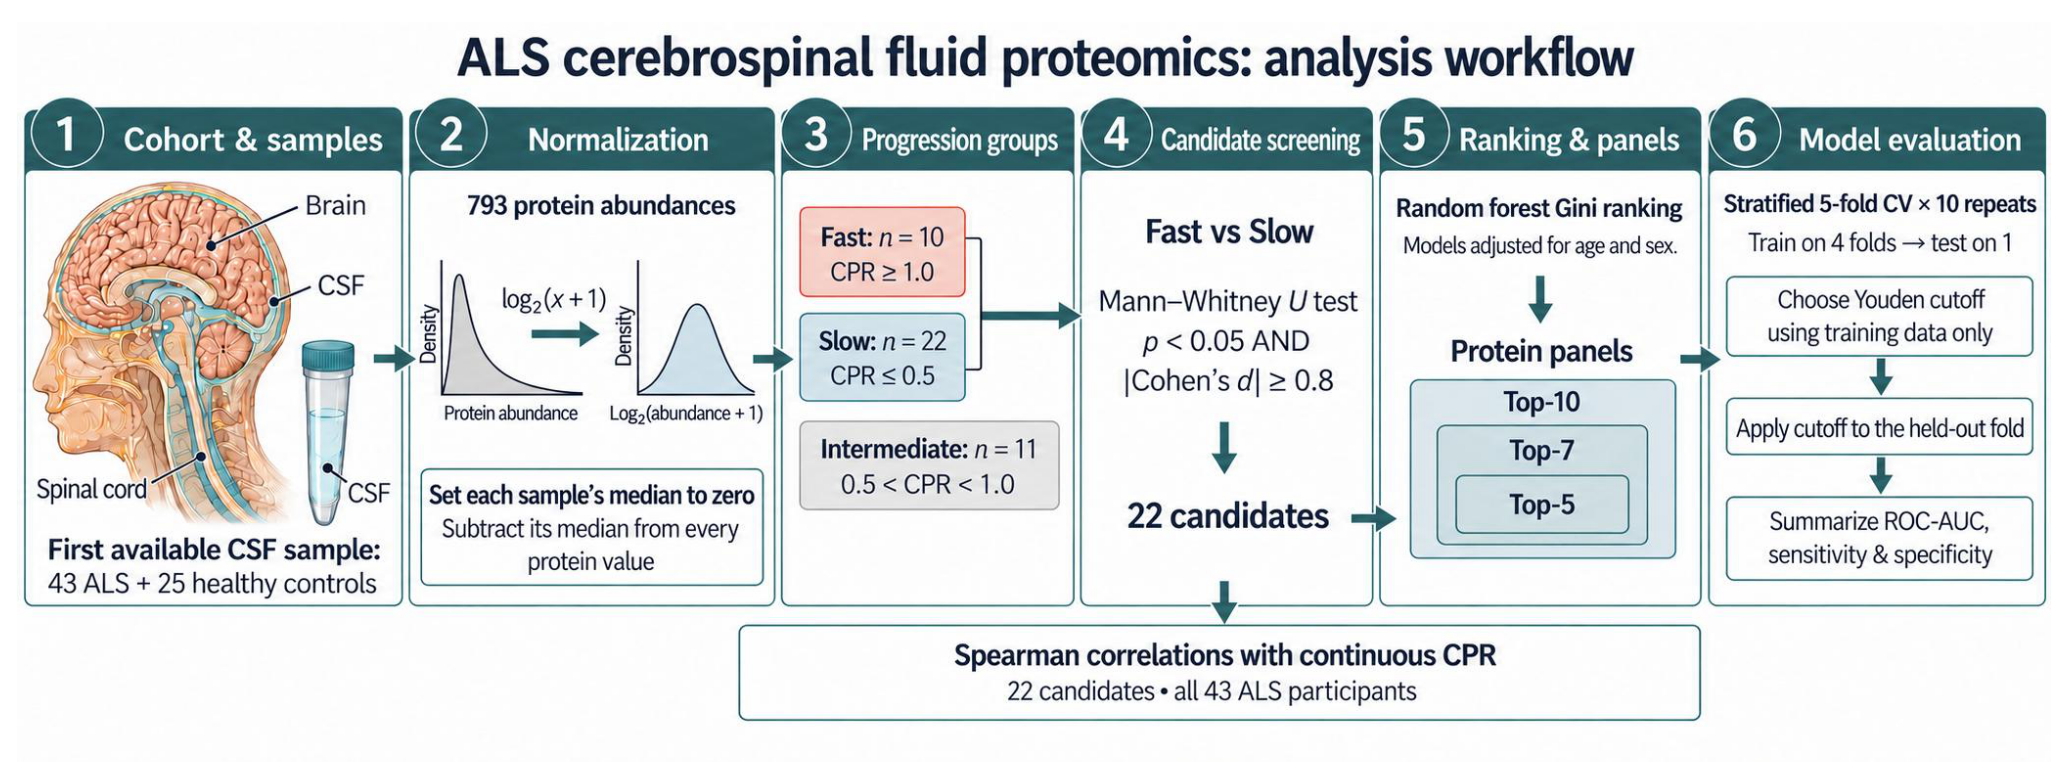
\includegraphics[width=\textwidth]{fig1_workflow.png}
\caption{Analysis workflow. First available CSF samples from 43 ALS participants and 25 healthy controls were log-transformed and median-centered. Fast ($n = 10$) and Slow ($n = 22$) participants were compared to select 22 candidate proteins, which were ranked by random forest importance to form Top-5, Top-7, and Top-10 panels and evaluated by repeated cross-validation. Candidates were also correlated with continuous CPR in all 43 ALS participants.}
\label{fig:workflow}
\end{figure}

\subsection{Clinical progression rate and outcome groups}

The ALSFRS-R rates function from 48 (normal function) to 0 (maximal impairment on the scale) \citep{cedarbaum1999}. The clinical field \texttt{Rate.of.progression} agreed to numerical precision in all 43 ALS participants with
\[
\text{CPR} = \frac{48 - \text{ALSFRS-R}}{\text{months from symptom onset}}.
\]
CPR estimates the average loss in ALSFRS-R points per month from reported symptom onset to the sampled visit. Participants were labeled \emph{Fast} when $\text{CPR} \geq 1.0$, \emph{Slow} when $\text{CPR} \leq 0.5$, and \emph{Intermediate} when $0.5 < \text{CPR} < 1.0$. Screening and binary classification used the 10 Fast and 22 Slow participants. Continuous CPR analysis included all 43 ALS participants, including the 11 Intermediate cases.

Disease duration was excluded from model predictors because it is part of the CPR formula. Duration at CSF collection was reported descriptively and considered when interpreting the protein differences.

\subsection{Proteomic preprocessing}

Abundance values were transformed as $\log_2(x+1)$ to reduce right skew. For each CSF sample, the median across all 793 measured proteins was then subtracted from every transformed protein value. This sample-wise median centering reduced between-sample differences in overall level without using the progression label. The effect of preprocessing was checked by plotting abundance distributions and sample medians before and after each step (Figure~\ref{fig:preprocessing}).

\begin{figure}[H]
\centering
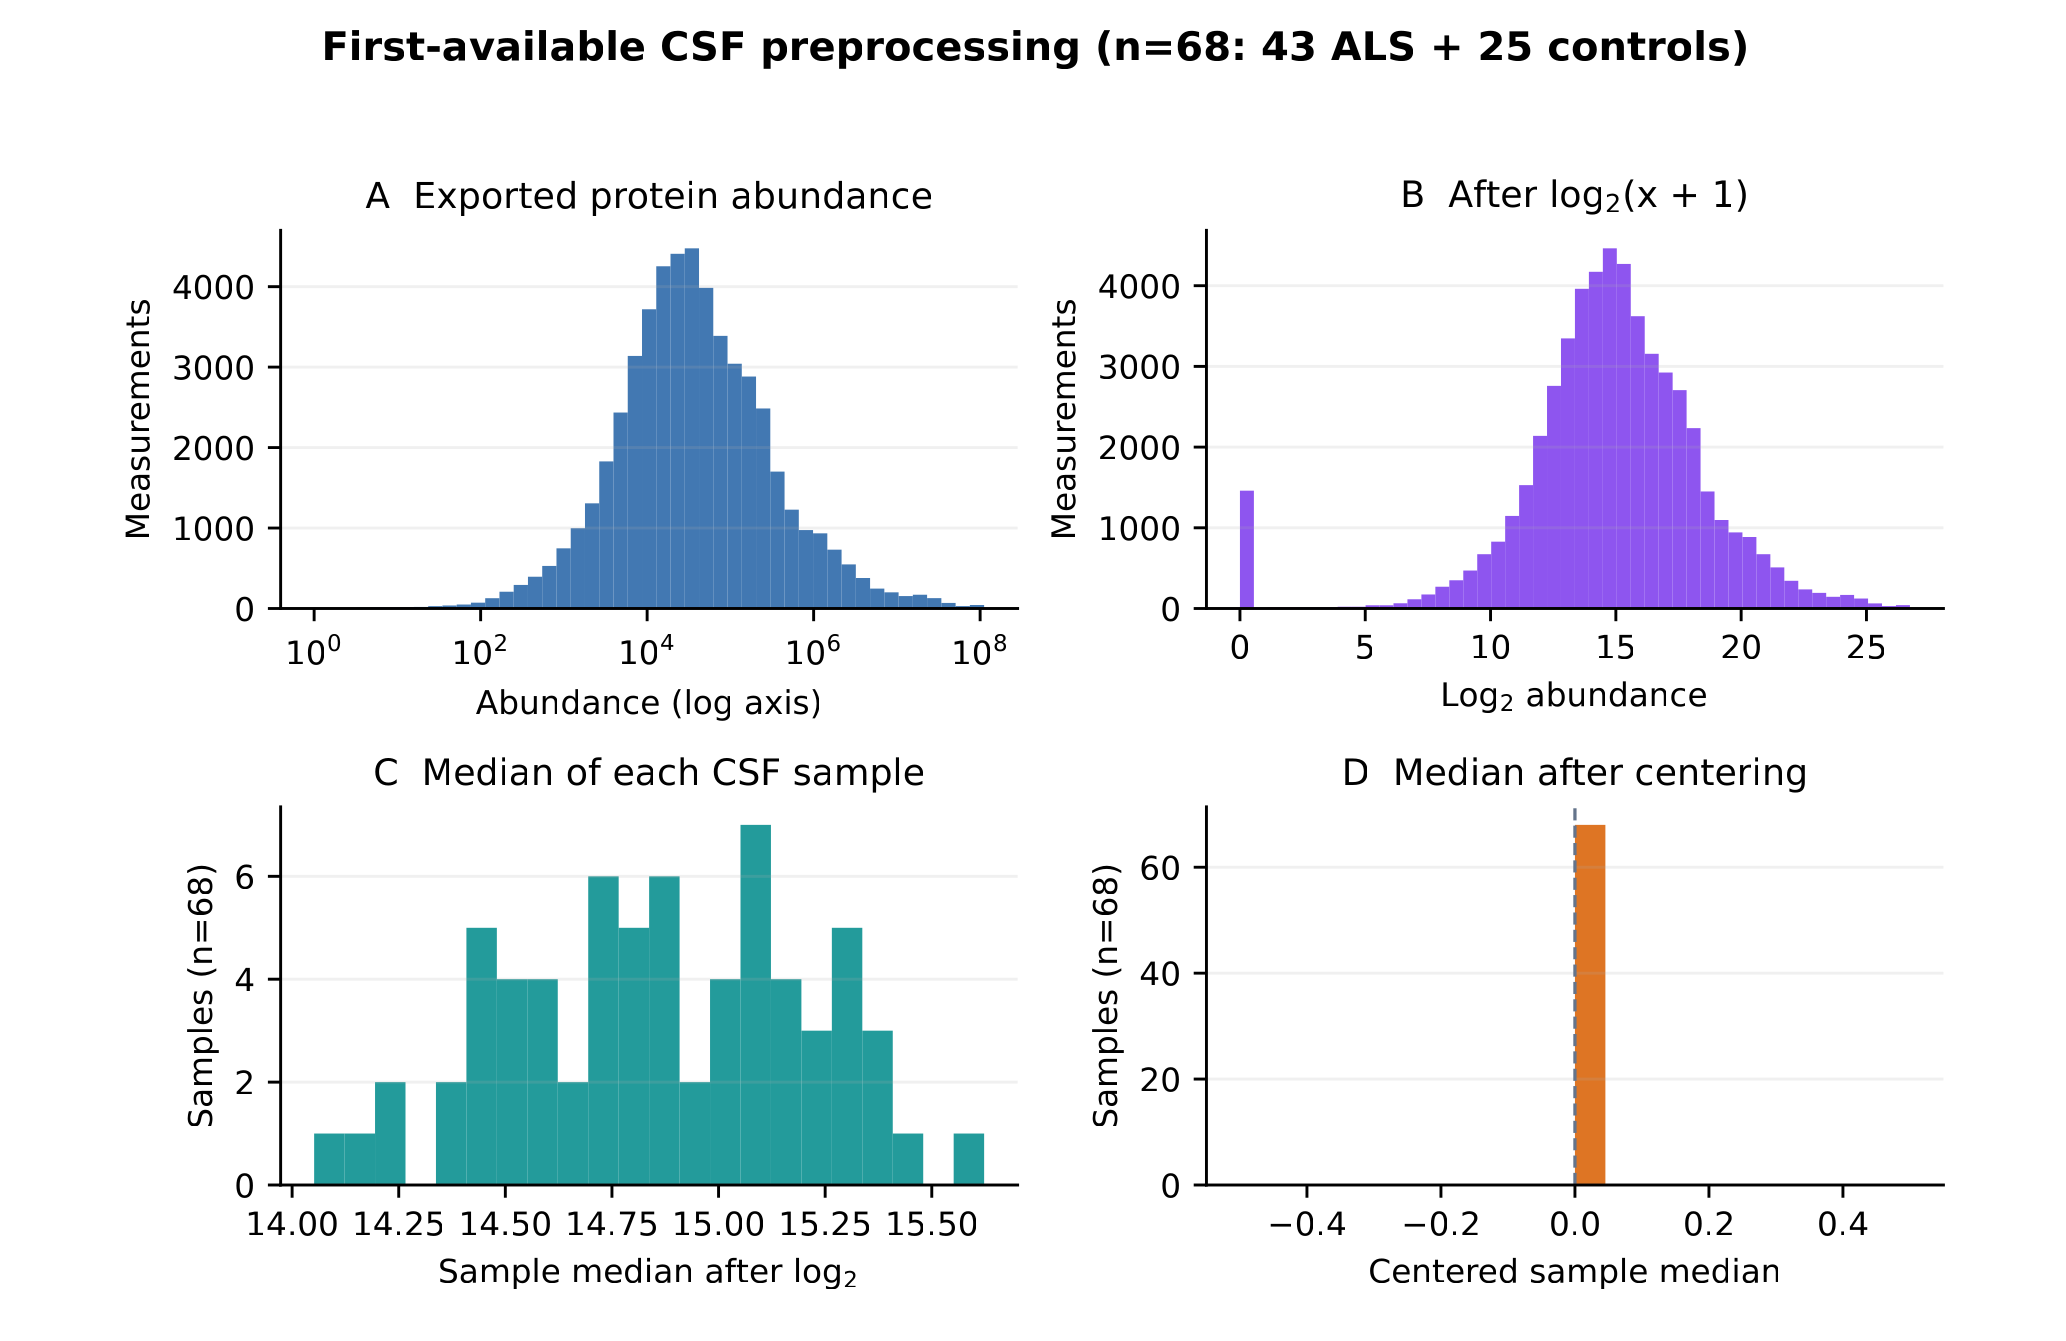
\includegraphics[width=\textwidth]{fig2_preprocessing.png}
\caption{Proteomic preprocessing quality control. (A) Exported abundance distribution on a logarithmic axis. (B) Distribution after $\log_2(x+1)$ transformation. (C) CSF-sample medians after log transformation. (D) Sample medians after median-centering, showing alignment around zero.}
\label{fig:preprocessing}
\end{figure}

\subsection{Protein screening and continuous CPR associations}

Each of the 793 proteins was compared between the 10 Fast and 22 Slow participants using a two-sided Mann--Whitney U test. Cohen's $d$ measured the mean normalized abundance difference (Fast minus Slow) divided by the pooled standard deviation. Candidate selection required both
\[
p_{\text{MWU}} < 0.05 \quad \text{and} \quad |d| \geq 0.8,
\]
combining nominal statistical significance with a large estimated group difference. Benjamini--Hochberg false discovery rate (FDR) correction was also calculated across all 793 tests \citep{benjamini1995}. No protein met the proteome-wide $q < 0.05$ criterion, so the dual screen was used for exploratory candidate selection.

For the 22 selected proteins, Spearman correlations with continuous CPR were calculated across all 43 ALS participants, and associations with $|\rho| \geq 0.40$ and $p < 0.05$ were highlighted. A positive $\rho$ indicates higher protein abundance with faster progression; a negative $\rho$ indicates the reverse. Benjamini--Hochberg $q$-values were calculated across these 22 tests. Because the same participants were used to select the candidates, these $q$-values are not independent confirmation. Correlations were not adjusted for age or sex.

\subsection{Random forest models, covariates, and panel construction}

All random forests used 100 trees, maximum depth 5, minimum split size 5, minimum leaf size 2, and Fast:Slow class weights of 3:1. Age at the first CSF visit (in years) and sex (male = 1, female = 0) were included as additional predictors in every model, so each panel used its specified number of proteins plus age and sex.

A ranking forest containing all 22 selected proteins plus age and sex was fitted to the full 32-participant Fast--Slow cohort. Proteins were ordered by Gini importance, which measures how much a feature improves Fast--Slow separation across the forest's decision-tree splits \citep{breiman2001}. Only protein importances determined panel membership. The five, seven, and ten highest-ranked proteins formed nested Top-5, Top-7, and Top-10 panels, so each larger panel included every protein in the smaller one. The CD163 feature was annotated as scavenger receptor cysteine-rich type 1 protein M130 in the data. Two candidate features carry a ``-2'' suffix because the data quantified them as isoform~2 of their protein (UniProt accessions P56192-2 for MARS1 and O75326-2 for SEMA7A). SEMA7A-2 was measured separately from the main SEMA7A feature but shared most of its peptides with it (2 of 12 peptides were unique). Panel membership and the ranking are reported in Table~\ref{tab:panels} and Figure~\ref{fig:importance}.

\subsection{Repeated cross-validation}

Each panel was tested with stratified five-fold cross-validation. The 32 Fast and Slow participants were divided into five groups (folds), each containing two Fast and four or five Slow participants, so every fold had roughly the same mix as the full cohort. A model was trained on four folds and then predicted the fifth, and this was repeated until every participant had been predicted by a model that had never seen them during training. Class imbalance was handled with the class weights described above rather than by duplicating or removing participants.

This whole procedure was repeated 10 times with different random divisions, giving 50 train--test splits. All three panels used exactly the same splits, so differences between panels reflect the proteins rather than which participants happened to be in which fold. No participant had missing protein, age, or sex values.

Performance was measured with the area under the receiver operating characteristic curve (AUC). AUC is the probability that a randomly chosen Fast participant receives a higher predicted Fast probability than a randomly chosen Slow participant: 0.5 means no better than chance, and 1.0 means perfect separation. The main result for each panel is the average AUC across the 10 repeats, with the standard deviation (SD) showing how much that AUC changed from one repeat to the next. As a secondary check, each participant's 10 predicted probabilities were averaged and a single AUC was calculated from those averages.

\subsection{Choosing the classification cutoff}

The random forest gives each participant a probability of being a Fast progressor. Turning that probability into a Fast or Slow label requires a cutoff. A low cutoff catches more Fast progressors but mislabels more Slow ones; a high cutoff does the reverse. Youden's $J$ scores each possible cutoff by how well it balances the two:
\[
J = \text{sensitivity} + \text{specificity} - 1,
\]
where sensitivity is the fraction of Fast participants labeled Fast and specificity is the fraction of Slow participants labeled Slow. $J$ equals 0 for a cutoff that does no better than guessing and 1 for perfect separation. In each of the 50 training sets, the cutoff with the highest $J$ was found using only the training participants, through a second, inner five-fold cross-validation. That cutoff was then applied unchanged to the held-out participants. Because the cutoff never saw the test participants, it could not be tuned to fit them.

Each participant therefore received 10 Fast/Slow labels, one per repeat. Their final label was the majority vote; in a 5--5 tie, the label went to whichever side of the cutoff their probabilities fell on average. Sensitivity, specificity, balanced accuracy (the average of sensitivity and specificity), and overall accuracy were calculated from these final labels.

\subsection{Software and data availability}

Analyses were performed in Python using pandas, NumPy, SciPy, scikit-learn, and matplotlib. Analysis code, aggregate results, and the manuscript figures are available in the accompanying repository (\url{https://github.com/princeote/als-csf-progression-biomarker-analysis}). The source mass-spectrometry data are publicly available in the PRIDE archive under accession PXD024219 (\url{https://www.ebi.ac.uk/pride/archive/projects/PXD024219}) \citep{perezriverol2022}. The participant-level clinical and intensity tables used here cannot be redistributed under the data use agreement; requests should be directed to the source study team \citep{thompson2021}.

% ------------------------------------------------------------------
\section{Results}
% ------------------------------------------------------------------

\subsection{Cohort characteristics}

The cohort included 43 ALS participants: 10 Fast, 22 Slow, and 11 Intermediate (Table~\ref{tab:cohort}). Fast and Slow groups did not differ significantly in age, sex, ALSFRS-R score, or onset site. Median disease duration at CSF collection was 7.0 months for Fast and 37.5 months for Slow participants ($p < 0.0001$), which is expected because duration is part of the CPR formula.

\begin{table}[H]
\centering
\footnotesize
\setlength{\tabcolsep}{4pt}
\begin{tabular}{>{\raggedright\arraybackslash}p{3.1cm}*{4}{>{\centering\arraybackslash}p{2.45cm}}>{\centering\arraybackslash}p{1.5cm}}
\toprule
Characteristic & ALS total ($n=43$) & \emph{Fast} ($n=10$) & \emph{Slow} ($n=22$) & \emph{Intermediate} ($n=11$) & Fast--Slow $p$ \\
\midrule
Female sex, $n$ (\%) & 12 (27.9) & 3 (30.0) & 6 (27.3) & 3 (27.3) & 1.000 \\
Age at visit, median years (IQR) & 62.7 (55.2--69.3) & 66.2 (62.8--68.7) & 62.6 (56.5--69.4) & 56.2 (51.9--66.5) & 0.699 \\
Duration at CSF, median months (IQR) & 21.3 (14.1--37.5) & 7.0 (5.7--10.0) & 37.5 (28.1--77.4) & 17.9 (14.7--22.0) & $<0.0001$ \\
ALSFRS-R, median (IQR) & 36.0 (33.0--38.5) & 36.0 (31.2--39.5) & 35.5 (33.2--39.5) & 36.0 (34.5--37.5) & 0.713 \\
CPR, median points/month (IQR) & 0.496 (0.283--0.949) & 1.285 (1.200--1.726) & 0.283 (0.165--0.427) & 0.617 (0.582--0.687) & N/A \\
Bulbar/limb onset, $n$ & 8/35 & 2/8 & 3/19 & 3/8 & 0.637 \\
\bottomrule
\end{tabular}
\caption{Cohort characteristics. Continuous Fast--Slow comparisons used two-sided Mann--Whitney U tests; categorical comparisons used two-sided Fisher exact tests. CPR was not tested because it defines the progression groups. Disease duration is descriptive and was not a classifier predictor. IQR, interquartile range ($Q_1$--$Q_3$); ALSFRS-R, ALS Functional Rating Scale--Revised; CPR, Clinical Progression Rate.}
\label{tab:cohort}
\end{table}

\subsection{Protein screen}

Twenty-two of 793 proteins met both $p < 0.05$ and $|d| \geq 0.8$ (Figure~\ref{fig:volcano}). The direction of $d$ is Fast minus Slow: positive values indicate greater normalized abundance among Fast participants and negative values indicate lower abundance. No protein passed Benjamini--Hochberg $q < 0.05$, so the screen narrowed the candidates but did not establish proteome-wide significance.

\begin{figure}[H]
\centering
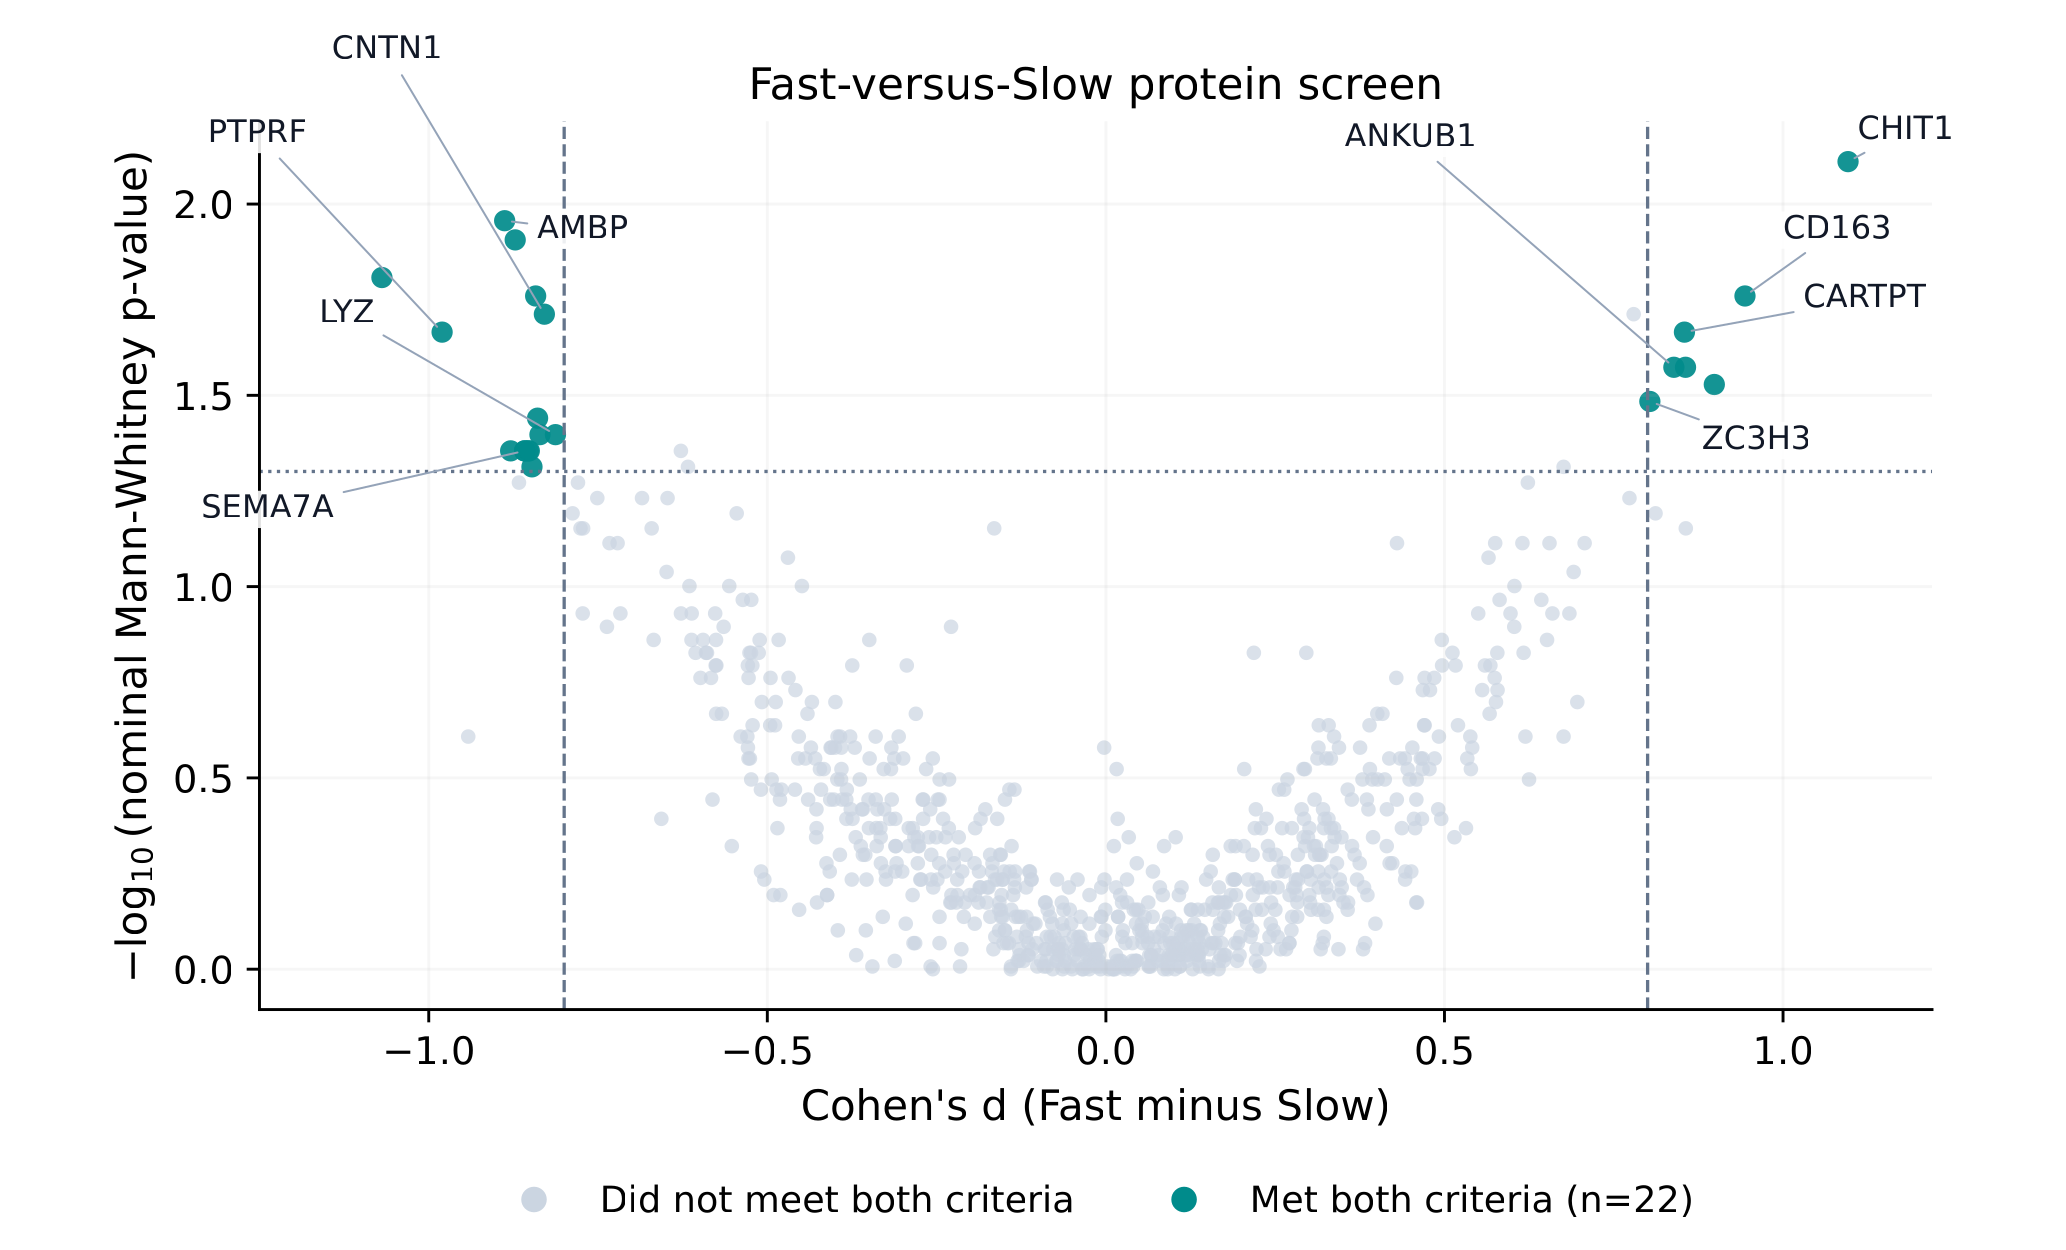
\includegraphics[width=0.92\textwidth]{fig3_volcano.png}
\caption{Fast-versus-Slow protein screen. Gray points failed at least one requirement. Teal points passed both nominal $p < 0.05$ and $|d| \geq 0.8$ and formed the candidate set. Dashed vertical lines mark $|d| = 0.80$ and the dotted horizontal line marks nominal $p = 0.05$. Labels identify the Top-10 panel proteins. No protein survived BH correction across 793 tests.}
\label{fig:volcano}
\end{figure}

\subsection{Continuous CPR associations}

Four screen-positive proteins also had $|\rho| \geq 0.40$ and $p < 0.05$ across all 43 ALS participants (Figure~\ref{fig:cpr}). CHIT1 showed the strongest positive association ($\rho = 0.522$, nominal $p = 0.00033$, $q = 0.00726$), followed by CD163 ($\rho = 0.446$, $p = 0.00274$, $q = 0.0233$) and ZC3H3 ($\rho = 0.422$, $p = 0.00483$, $q = 0.0266$). ITIH5 was inversely associated with CPR ($\rho = -0.440$, $p = 0.00318$, $q = 0.0233$). All four met $q < 0.05$ within the 22 candidate correlation tests. ITIH5 was outside the Top-10 panel, showing that continuous association and classifier ranking capture different aspects of the data.

\begin{figure}[H]
\centering
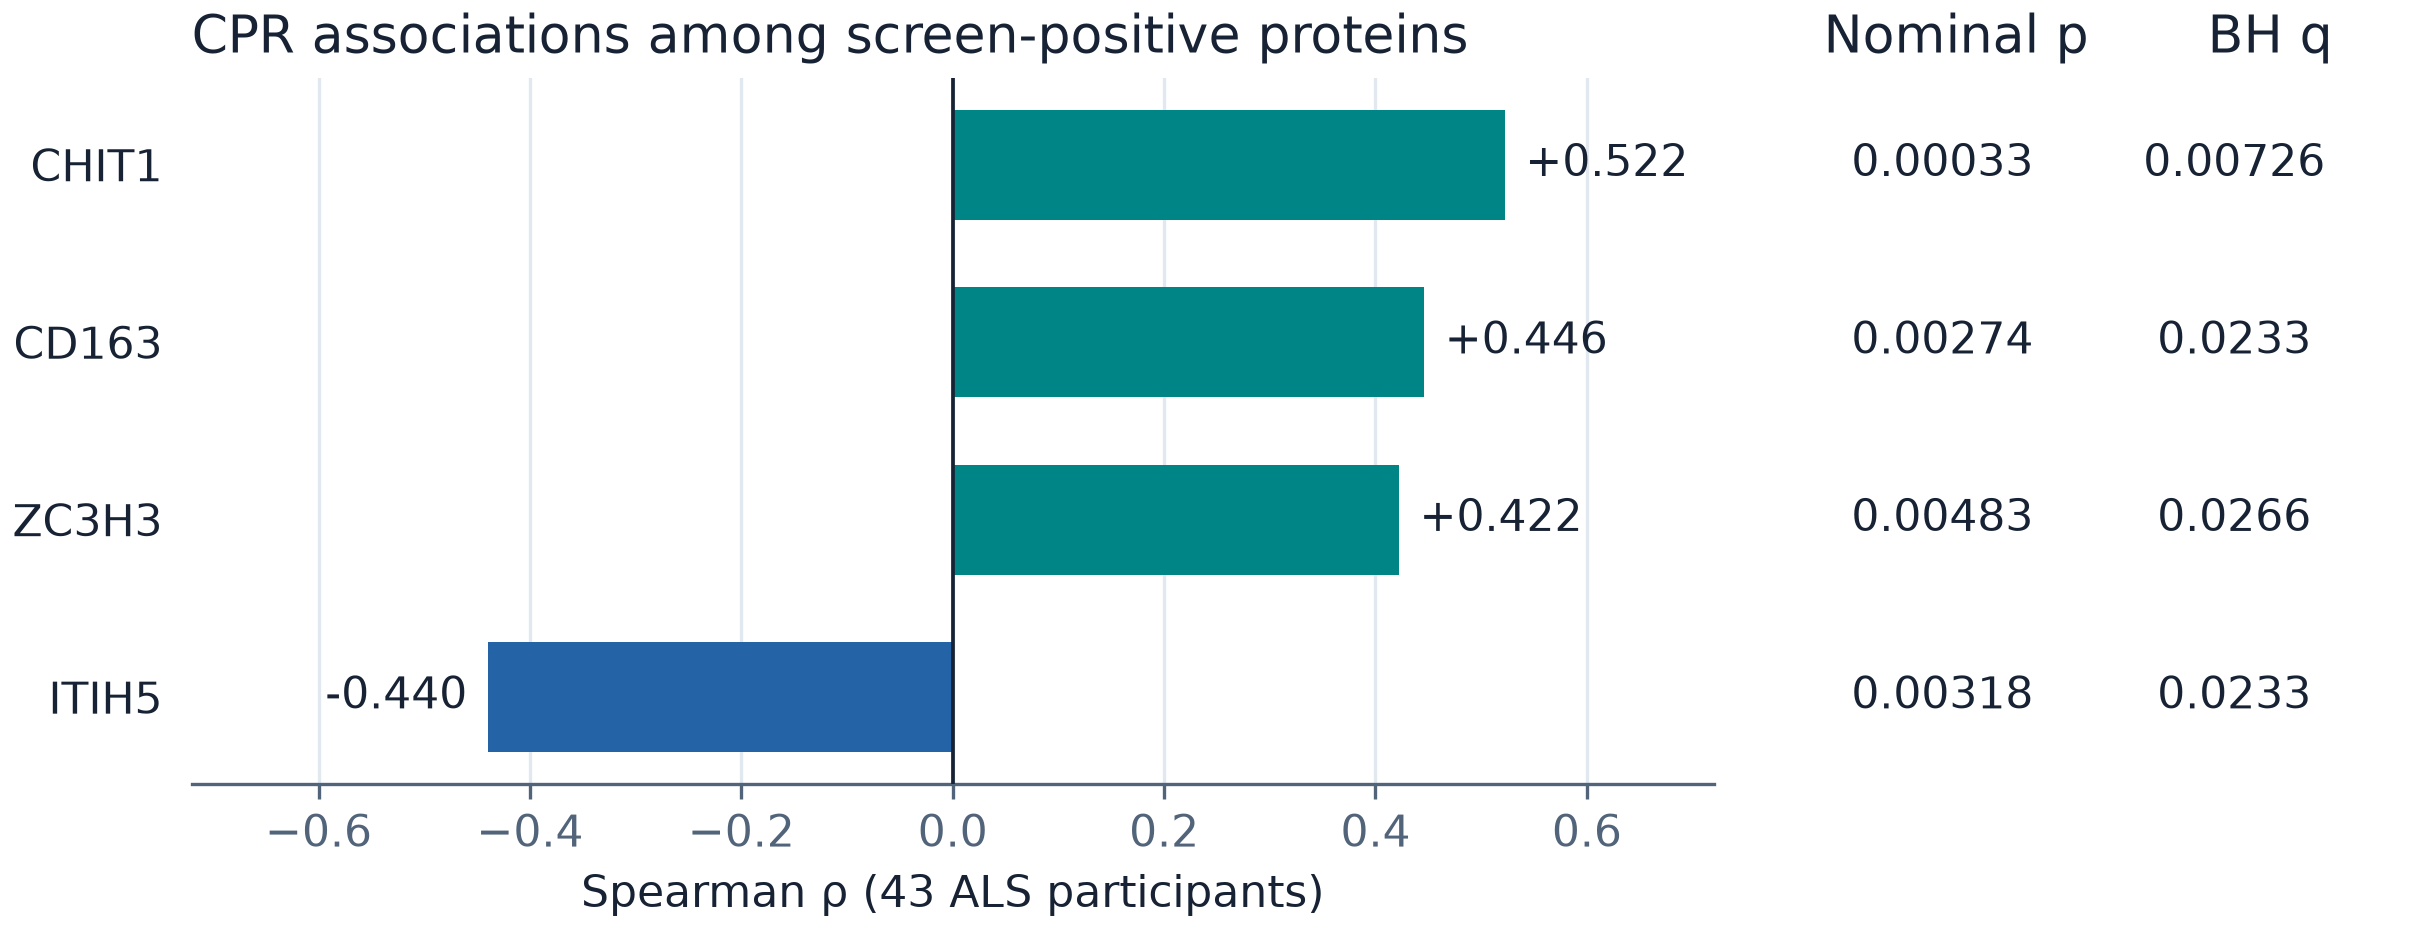
\includegraphics[width=0.92\textwidth]{fig4_cpr_summary.png}
\caption{Spearman correlations with continuous CPR for the four screen-positive proteins that met $|\rho| \geq 0.40$ and nominal $p < 0.05$. The correlations use all 43 ALS participants, including Intermediate cases, and are unadjusted for age and sex. BH $q$-values correct across the 22 candidate correlation tests.}
\label{fig:cpr}
\end{figure}

\subsection{Random forest ranking and candidate panels}

Figure~\ref{fig:importance} shows the Gini importance of the 22 screen-positive proteins in a random forest that also included age and sex. The panels contained the five, seven, or ten highest-ranked proteins (Table~\ref{tab:panels}). Top-5 comprised CHIT1, ZC3H3, CNTN1, PTPRF, and ANKUB1. Top-7 added LYZ and CARTPT. Top-10 added CD163, AMBP, and SEMA7A.

\begin{figure}[H]
\centering
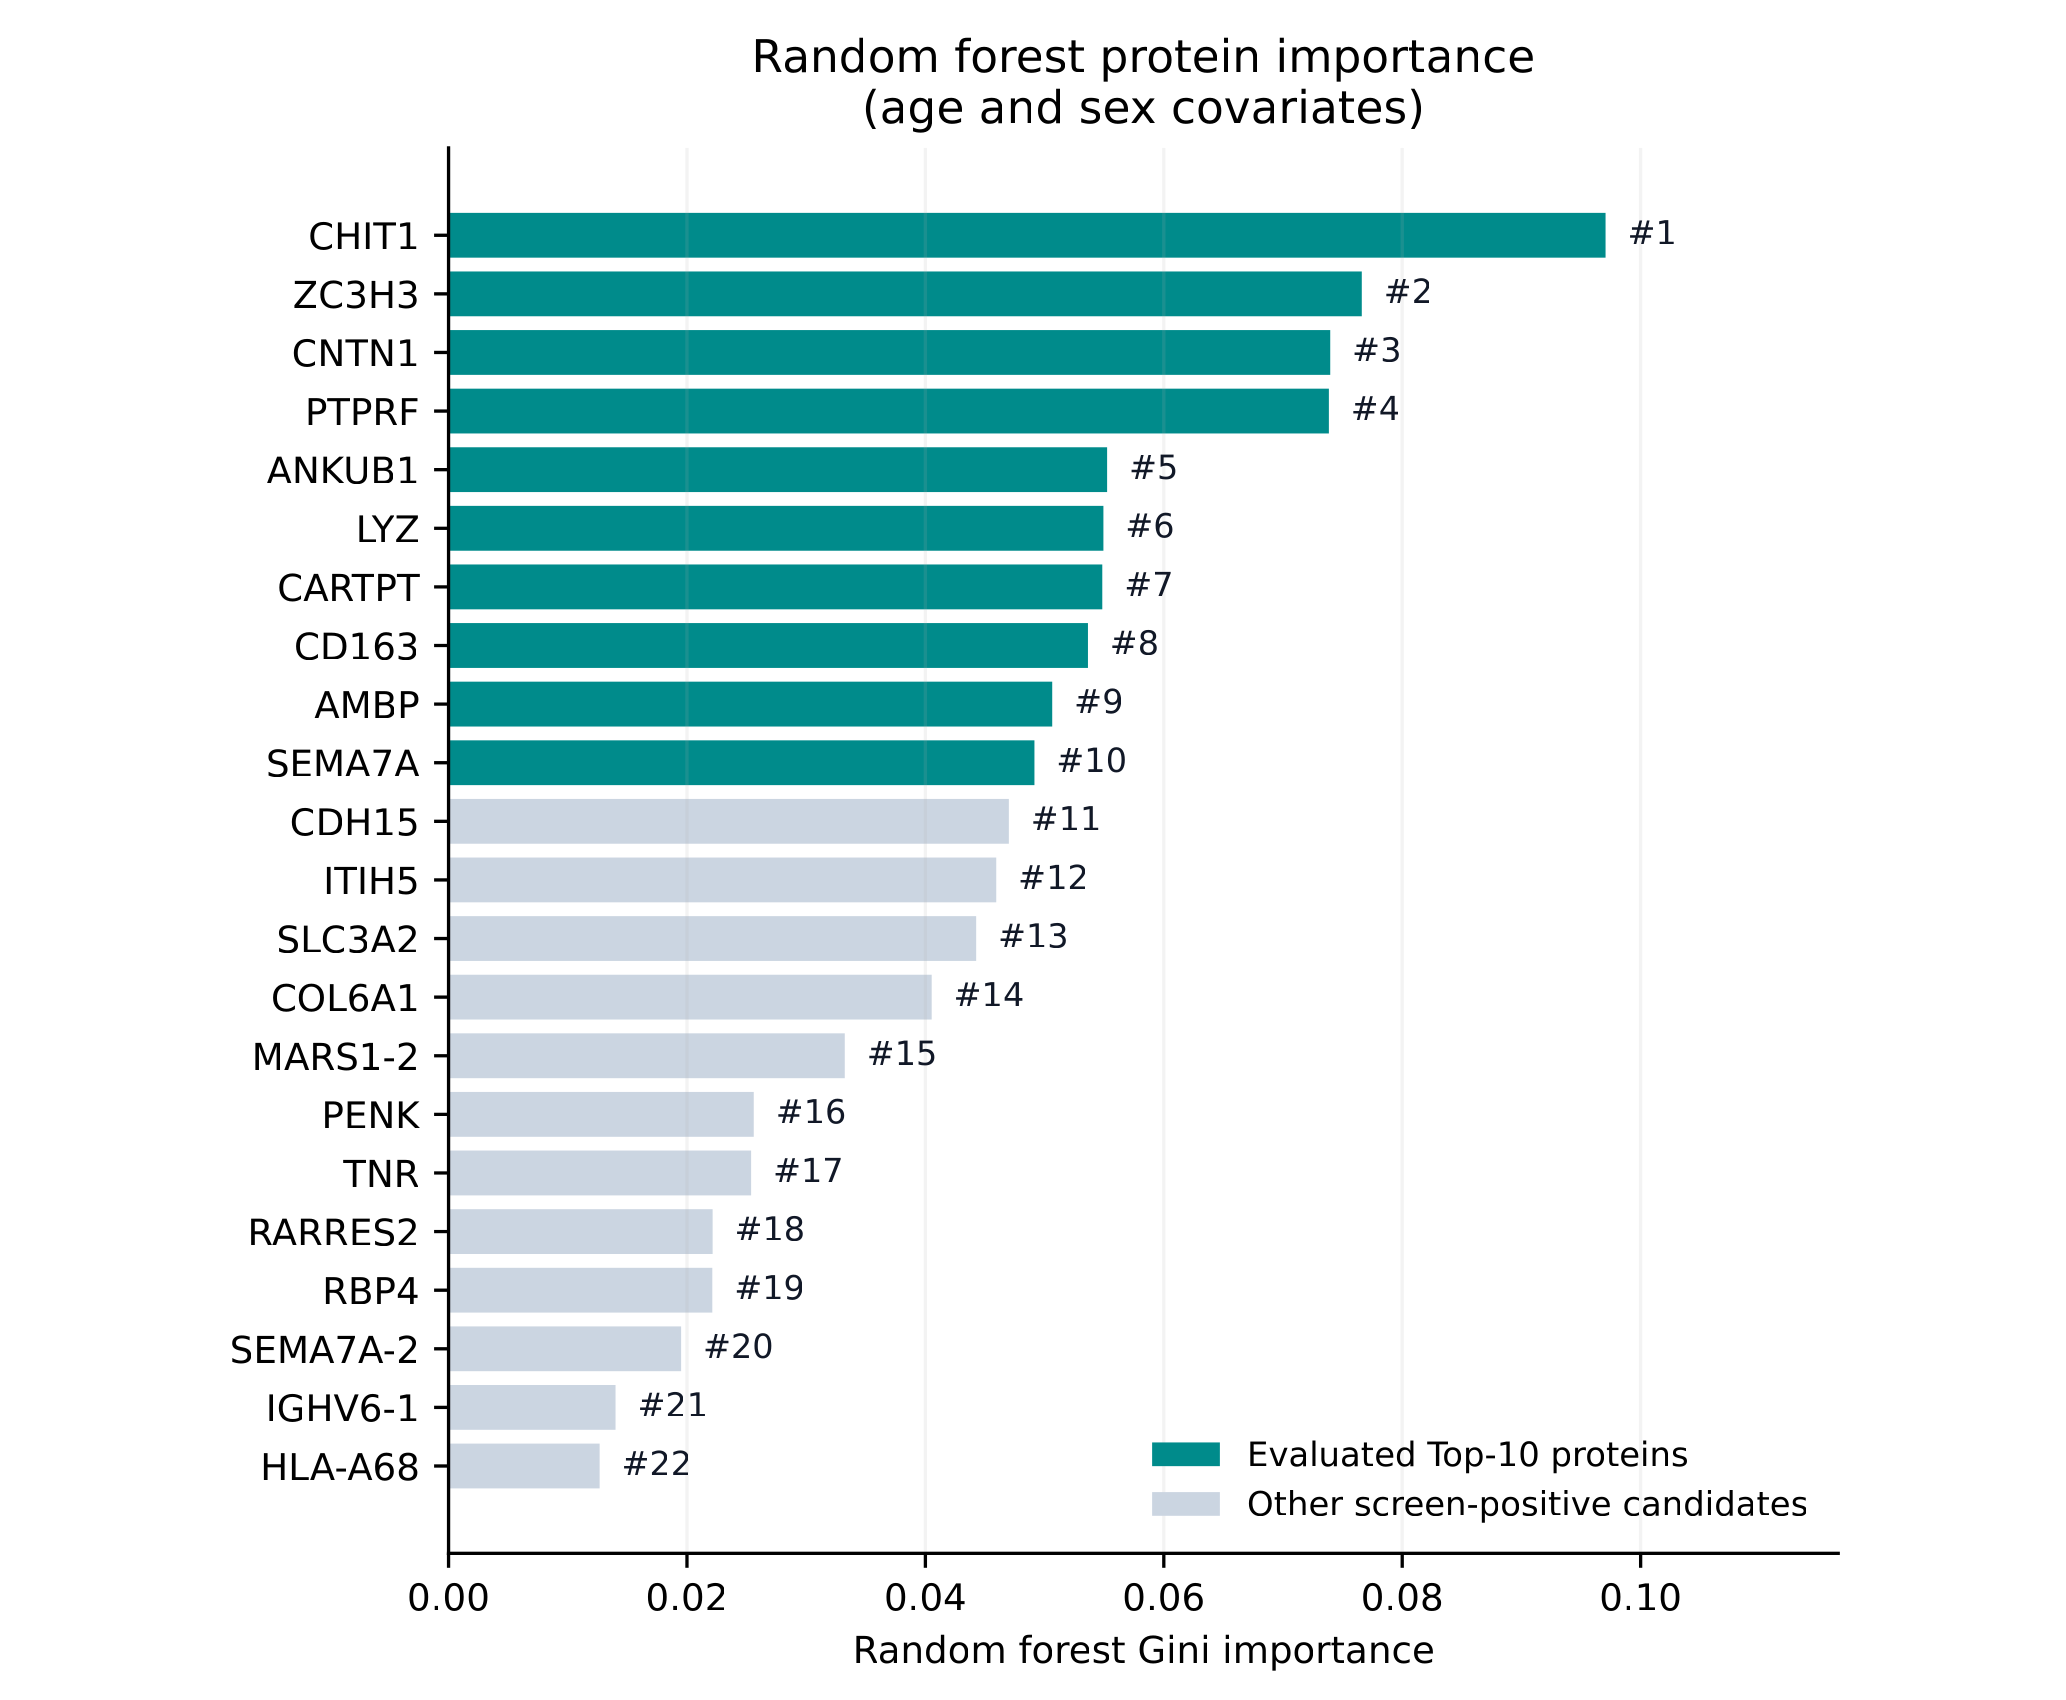
\includegraphics[width=0.85\textwidth]{fig5_importance.png}
\caption{Gini-importance ranking of the 22 screen-positive candidates from a random forest with age and sex as covariates. Bar length shows importance and the labels at the right give the rank. Teal bars identify the Top-10 panel; gray bars show the remaining candidates.}
\label{fig:importance}
\end{figure}

\begin{table}[H]
\centering
\small
\begin{tabular}{l>{\raggedright\arraybackslash}p{6.3cm}>{\raggedright\arraybackslash}p{5.2cm}}
\toprule
Panel & Proteins & Relationship to smaller panel \\
\midrule
Top-5 & CHIT1, ZC3H3, CNTN1, PTPRF, ANKUB1 & Five-protein candidate panel \\
Top-7 & CHIT1, ZC3H3, CNTN1, PTPRF, ANKUB1, LYZ, CARTPT & Top-5 plus LYZ and CARTPT \\
Top-10 & CHIT1, ZC3H3, CNTN1, PTPRF, ANKUB1, LYZ, CARTPT, CD163, AMBP, SEMA7A & Top-7 plus CD163, AMBP, and SEMA7A \\
\bottomrule
\end{tabular}
\caption{Candidate-panel definitions from the random forest ranking. Age and sex are additional model covariates in every panel.}
\label{tab:panels}
\end{table}

\subsection{Protein-level evidence in the candidate panels}

All ten Top-10 proteins met the Fast-versus-Slow screen (Table~\ref{tab:proteins}; Figure~\ref{fig:protein-effects}). CHIT1, ZC3H3, ANKUB1, CARTPT, and CD163 had higher normalized abundance in Fast participants; CNTN1, PTPRF, LYZ, AMBP, and SEMA7A were lower. CHIT1 had the largest positive effect ($d = 1.10$) and PTPRF the largest negative effect ($d = -0.98$).

\begin{table}[H]
\centering
\begin{tabular}{rlrrrrr}
\toprule
Rank & Protein & MWU $p$ & Cohen's $d$ & CPR $\rho$ & CPR $p$ & CPR BH $q$ \\
\midrule
1 & CHIT1 & 0.00775 & 1.096 & 0.522 & 0.000330 & 0.00726 \\
2 & ZC3H3 & 0.0328 & 0.803 & 0.422 & 0.00483 & 0.0266 \\
3 & CNTN1 & 0.0194 & $-0.829$ & $-0.360$ & 0.0178 & 0.0784 \\
4 & PTPRF & 0.0216 & $-0.980$ & $-0.190$ & 0.221 & 0.305 \\
5 & ANKUB1 & 0.0267 & 0.839 & 0.275 & 0.0743 & 0.136 \\
6 & LYZ & 0.0401 & $-0.813$ & $-0.161$ & 0.303 & 0.351 \\
7 & CARTPT & 0.0216 & 0.854 & 0.286 & 0.0634 & 0.136 \\
8 & CD163 & 0.0174 & 0.944 & 0.446 & 0.00274 & 0.0233 \\
9 & AMBP & 0.0111 & $-0.888$ & $-0.281$ & 0.0678 & 0.136 \\
10 & SEMA7A & 0.0442 & $-0.858$ & $-0.134$ & 0.393 & 0.393 \\
\bottomrule
\end{tabular}
\caption{Protein-level evidence for the Top-10 panel. Cohen's $d$ is Fast minus Slow, so its sign gives the direction of the group difference. MWU, two-sided Mann--Whitney U test. CPR correlations use all 43 ALS participants; CPR BH $q$ corrects across the 22 screen-positive proteins. No protein passed BH $q < 0.05$ across the 793 screening tests.}
\label{tab:proteins}
\end{table}

\begin{figure}[H]
\centering
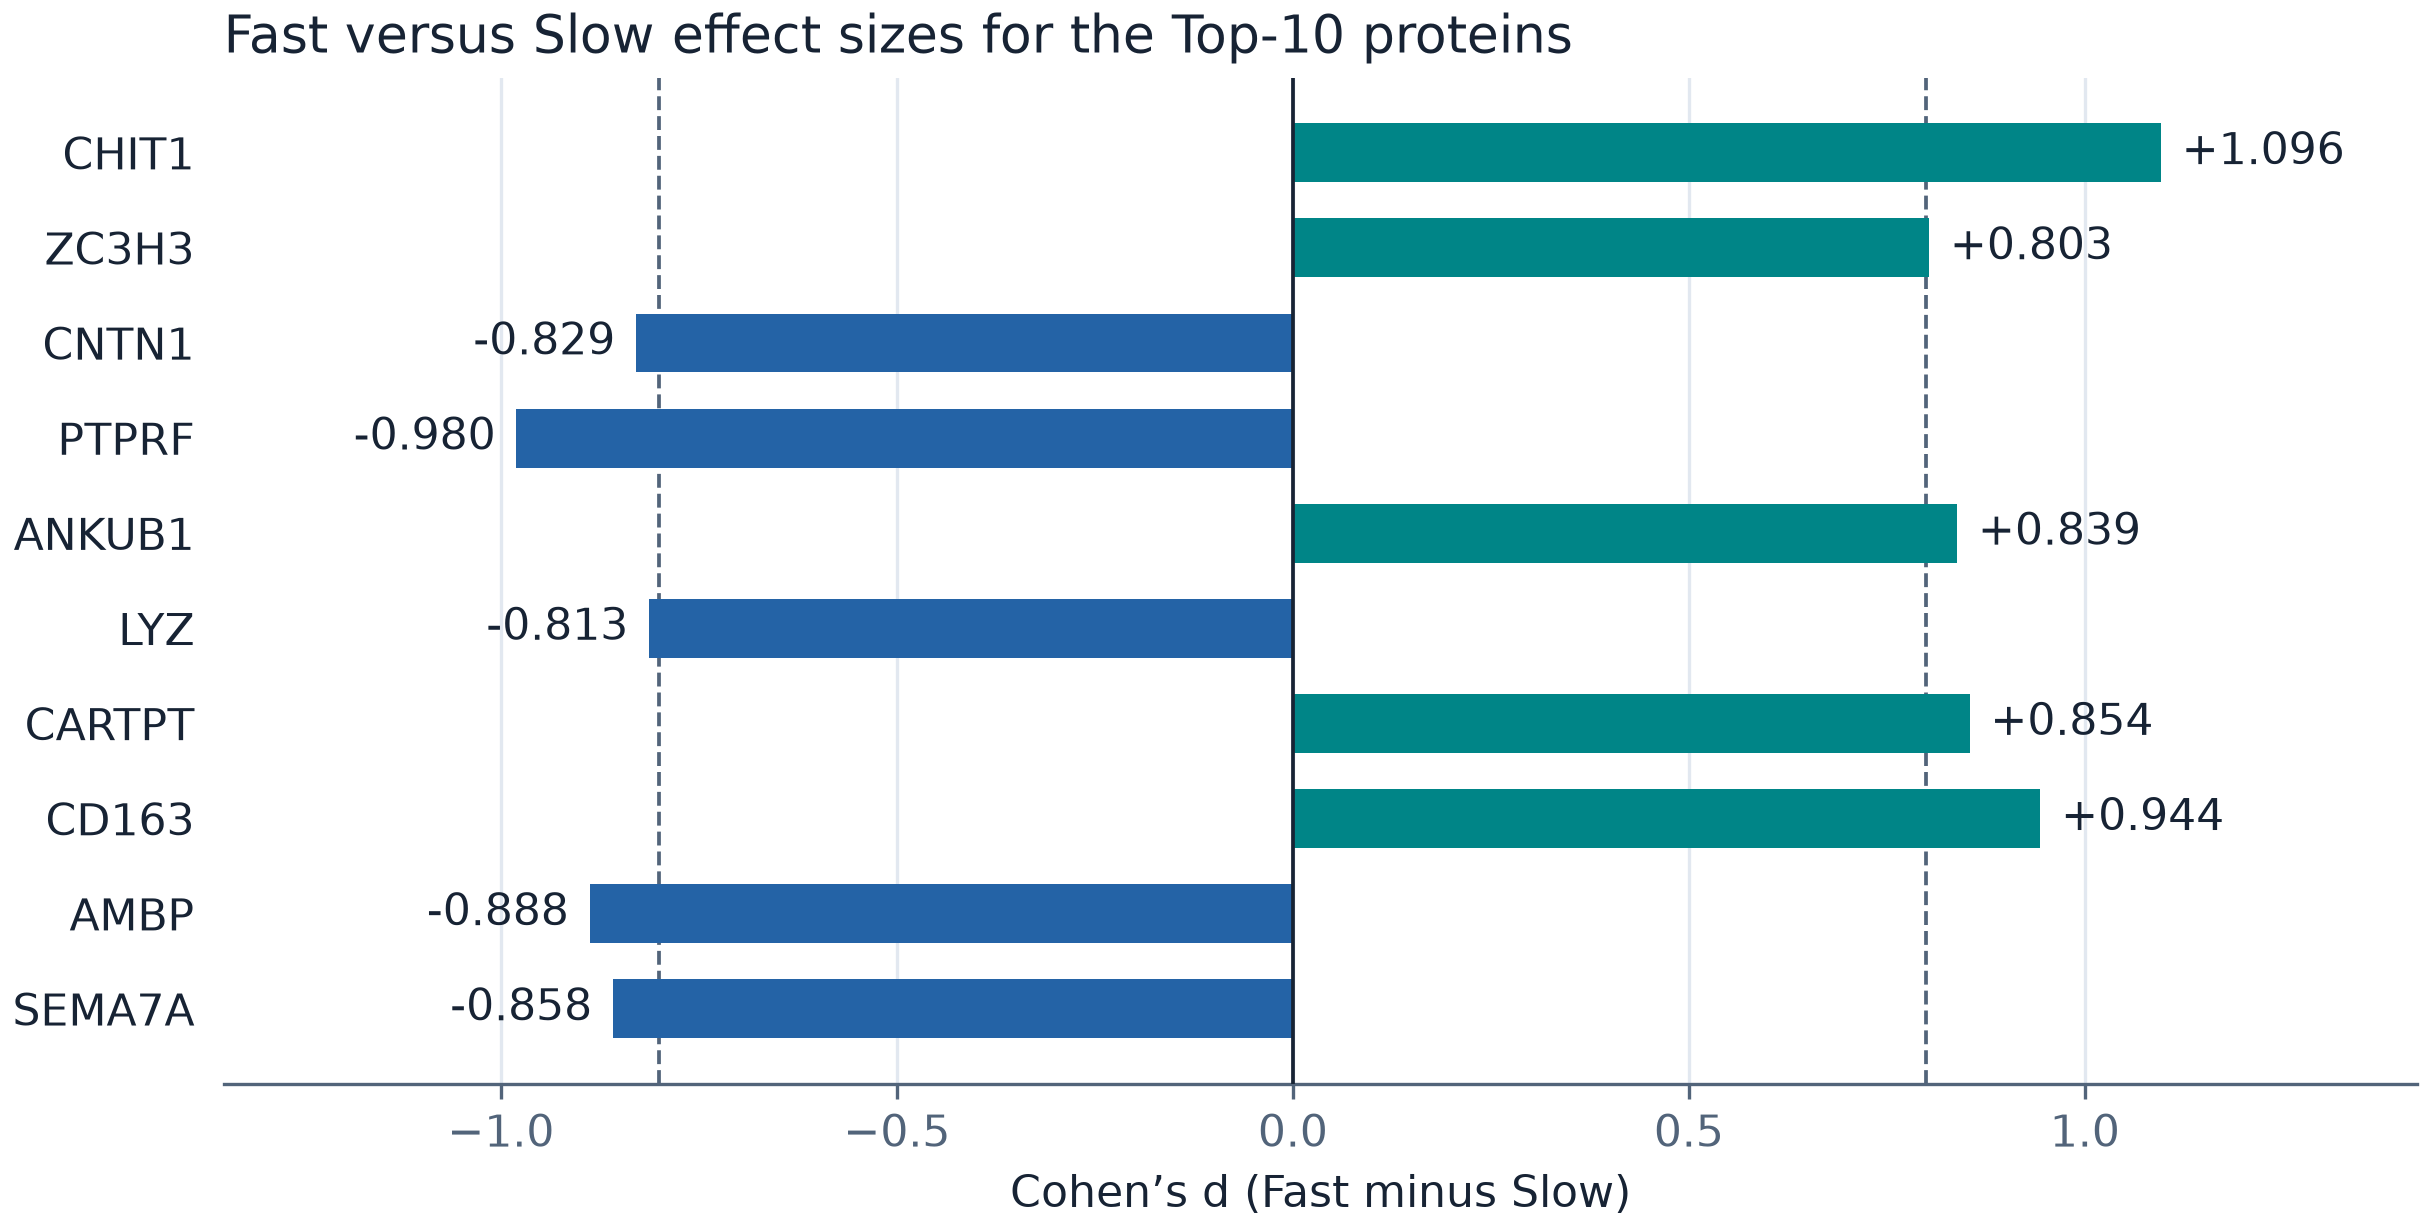
\includegraphics[width=\textwidth]{fig6_protein_effects.png}
\caption{Group-level standardized differences in normalized protein abundance for the Top-10 panel, ordered by Gini rank. Cohen's $d$ is Fast minus Slow. Dashed lines indicate the screening threshold of $|d| = 0.8$.}
\label{fig:protein-effects}
\end{figure}

\subsection{Repeated cross-validation and classification performance}

Average AUCs across the 10 repeats were $0.876 \pm 0.029$ for Top-5, $0.835 \pm 0.045$ for Top-7, and $0.849 \pm 0.038$ for Top-10 (Table~\ref{tab:performance}; Figure~\ref{fig:performance}). Repeat-level AUCs ranged from 0.832 to 0.927, 0.782 to 0.918, and 0.791 to 0.909, respectively. Top-5 scored higher than Top-7 in 8 of 10 repeats and higher than Top-10 in 7 of 10. AUCs from participant-averaged probabilities showed the same order (0.891, 0.841, and 0.855).

Using each participant's majority label, Top-5 correctly classified 7 of 10 Fast and 20 of 22 Slow participants, Top-7 classified 6 of 10 Fast and 18 of 22 Slow, and Top-10 classified 7 of 10 Fast and 16 of 22 Slow (Table~\ref{tab:performance}).

\begin{table}[H]
\centering
\small
\begin{tabular}{lccc}
\toprule
Panel & Repeat AUC, mean $\pm$ SD & Participant-averaged AUC & Threshold median (IQR width) \\
\midrule
Top-5 & $0.876 \pm 0.029$ & 0.891 & 0.505 (0.131) \\
Top-7 & $0.835 \pm 0.045$ & 0.841 & 0.551 (0.165) \\
Top-10 & $0.849 \pm 0.038$ & 0.855 & 0.502 (0.122) \\
\bottomrule
\end{tabular}

\vspace{8pt}
\begin{tabular}{lcccc}
\toprule
Panel & Fast sensitivity & Slow specificity & Balanced accuracy & Accuracy \\
\midrule
Top-5 & 70.0\% & 90.9\% & 80.5\% & 84.4\% \\
Top-7 & 60.0\% & 81.8\% & 70.9\% & 75.0\% \\
Top-10 & 70.0\% & 72.7\% & 71.4\% & 71.9\% \\
\bottomrule
\end{tabular}
\caption{Performance of the three panels (all models include age and sex). \emph{Repeat AUC:} average of the 10 repeat AUCs $\pm$ SD. \emph{Participant-averaged AUC:} AUC calculated from each participant's average predicted probability. \emph{Sensitivity, specificity, and accuracy:} based on each participant's majority label across the 10 repeats. \emph{Threshold:} median Youden cutoff chosen across the 50 training sets, with the interquartile-range width in parentheses.}
\label{tab:performance}
\end{table}

\begin{figure}[H]
\centering
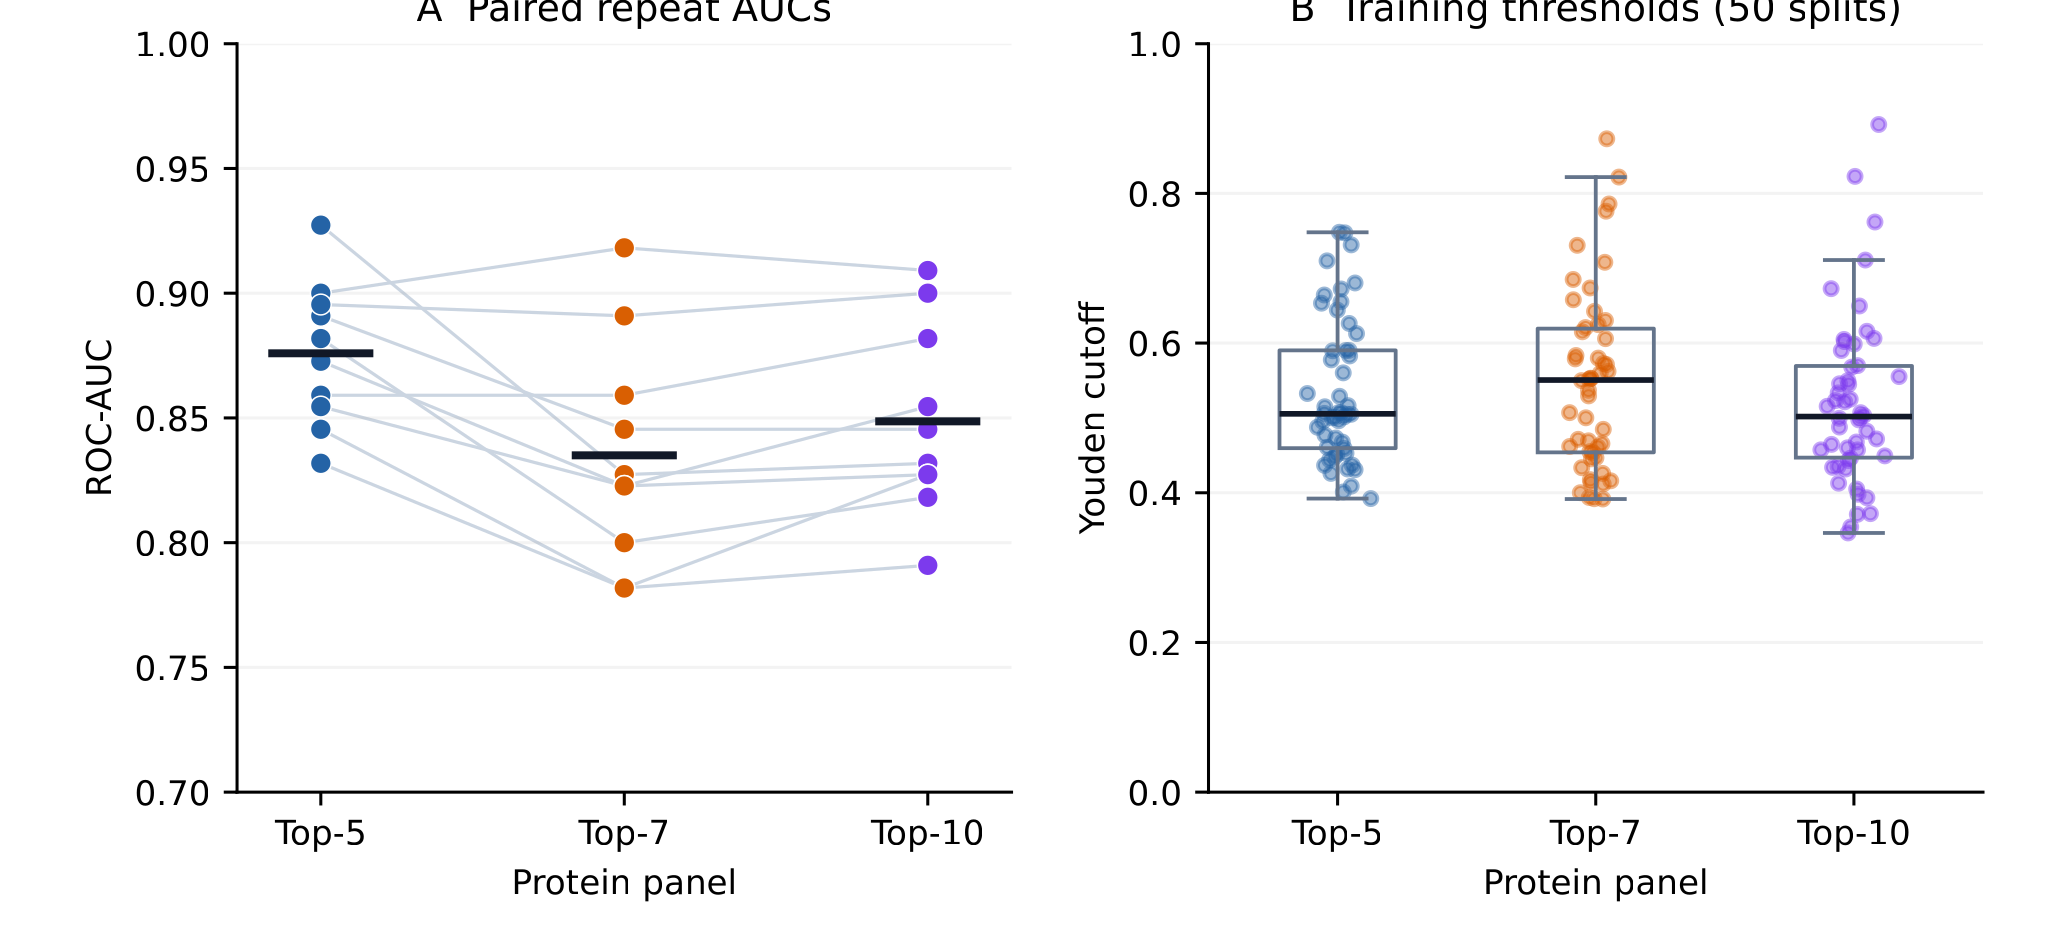
\includegraphics[width=\textwidth]{fig7_performance.png}
\caption{(A) AUC of each panel in each of the 10 repeats. Lines connect the three panels' results from the same repeat, which used identical training and test participants; black bars mark the averages. (B) Youden cutoff chosen in each of the 50 training sets. Boxes show the median and interquartile range; all three panels' cutoffs centered near 0.5.}
\label{fig:performance}
\end{figure}

% ------------------------------------------------------------------
\section{Discussion}
% ------------------------------------------------------------------

\subsection{Principal findings and panel comparison}

This study connected differences in ALS progression rate to specific CSF proteins. Twenty-two proteins differed between Fast and Slow participants, and four of them also tracked progression rate continuously across all 43 participants: CHIT1, CD163, and ZC3H3 were higher with faster progression, and ITIH5 was lower.

The continuous correlation adds information the group comparison cannot. First, it includes the 11 Intermediate participants who were left out of the Fast-versus-Slow comparison. It therefore tests whether a protein changes gradually with progression speed, not just whether it differs between the two extremes. A protein that rises steadily from slow to intermediate to fast progressors is more convincing than one that separates only the extremes, because a difference between two small groups can be driven by a few unusual participants. Second, progression in real patients is a continuum, not two categories, so a protein that tracks CPR is closer to how a marker would actually be used. For these reasons, CHIT1, CD163, ZC3H3, and ITIH5 are the strongest candidates for follow-up, although both analyses come from the same participants.

The Top-5 panel had the highest average AUC ($0.876 \pm 0.029$) and correctly classified 7 of 10 Fast and 20 of 22 Slow participants (70.0\% sensitivity, 90.9\% specificity). Adding proteins did not improve performance: Top-7 identified fewer Fast participants (60.0\%), and Top-10 identified fewer Slow participants (72.7\%).

Because only 10 of 32 participants were Fast, a model that labeled everyone Slow would already be 68.8\% accurate. Sensitivity, specificity, and balanced accuracy therefore describe performance better than accuracy alone. A five-protein panel is also far more practical to develop into a targeted clinical assay than a 793-protein discovery measurement.

\subsection{What the progression analyses capture}

The first available CSF sample provides a molecular snapshot that can be compared with the clinical picture at that visit, and a panel measured from one sample could eventually supply information without repeated lumbar punctures. Each participant's CSF was collected at a single visit, not always at diagnosis, and CPR measured how much function they had lost between symptom onset and that visit. These results therefore show which proteins are associated with how quickly a patient \emph{has} progressed. Whether the same proteins can predict how quickly a patient \emph{will} decline is a separate question, which requires following patients after their sample is taken. Repeated sampling could also help separate stable progression-associated signals from proteins that change with disease stage or treatment.

CHIT1 and ZC3H3 were in Top-5, CD163 was eighth-ranked, and ITIH5 was outside Top-10 despite its inverse CPR association. A correlation evaluates one protein at a time, whereas forest ranking reflects a protein's usefulness alongside other predictors for the binary classification task. A lower-ranked protein can therefore remain relevant to progression biology, and the differences between the two analyses help separate biological follow-up priorities from panel membership.

\subsection{Immune and RNA-processing candidates}

CHIT1 (chitotriosidase-1) was the highest-ranked protein, was more abundant in Fast participants ($d = 1.10$), and showed the strongest CPR correlation ($\rho = 0.52$). Prior CSF studies associate chitinases with ALS progression, and experimental work links CHIT1 to microglial or macrophage activation and neuroinflammatory injury \citep{thompson2019,varghese2020,steinacker2021}. Agreement between its group contrast and continuous correlation makes CHIT1 a biologically grounded candidate for investigating immune activity alongside functional decline.

CD163 was higher in Fast participants ($d = 0.94$) and correlated positively with CPR ($\rho = 0.45$), adding a second macrophage-associated candidate. CD163 participates in hemoglobin--haptoglobin clearance and innate immune sensing \citep{fabriek2009}. Published CSF evidence is assay-dependent: a small preselected-target data-independent acquisition study reported higher abundance in sporadic ALS, whereas another discovery-MS study could not detect CSF CD163 by enzyme-linked immunosorbent assay \citep{dellar2025,deluna2023}. % CHECK: confirm whether dellar2025 or dellar2024 is the DIA study that reported CD163.
This discrepancy makes confirmation of the detectable protein forms and measurement method an important next step for CD163.

ZC3H3 was second-ranked, was higher in Fast participants ($d = 0.80$), and correlated positively with CPR ($\rho = 0.42$). ZC3H3 participates in nuclear RNA polyadenylation and export \citep{hurt2009}, processes that help prepare messenger RNA and move it from the nucleus to the cytoplasm for protein production. This known function gives the association a specific RNA-processing context. The CSF measurement motivates testing whether ZC3H3 reproducibly tracks progression and determining its cellular source; it does not directly measure RNA-processing dysfunction in motor neurons.

\subsection{Neuronal adhesion and the remaining panel proteins}

CNTN1 (contactin-1) was lower in Fast participants ($d = -0.83$). It is a neuronal cell-adhesion molecule involved in organizing axonal membranes and the nodal regions between myelin segments, which support nerve-signal conduction \citep{colakoglu2014}. This function gives the observed CSF difference a clear connection to axonal organization. The CNTN1 measurement was annotated as a particular version (isoform) of contactin-1.

PTPRF was also lower in Fast participants ($d = -0.98$). It encodes the LAR receptor-type protein tyrosine phosphatase, which regulates signaling by removing phosphate groups from proteins. Experimental work in cultured hippocampal neurons implicated LAR in the organization and maintenance of excitatory synapses \citep{dunah2005}. This supplies a neuronal-signaling rationale for investigating PTPRF; lower CSF abundance does not itself demonstrate synaptic loss in ALS.

ANKUB1, the remaining Top-5 protein, was higher in Fast participants ($d = 0.84$). Its direct ALS-CSF literature is limited, so its contribution is currently statistical prioritization rather than a defined disease mechanism. Keeping it in the panel acknowledges that a feature can help discriminate groups before its biological meaning is established.

The Top-7 additions extended the range of biological questions. LYZ (lysozyme) was lower in Fast participants ($d = -0.81$) and provides an innate-immune candidate. It appeared in a prior ALS CSF discovery analysis but did not show significant differences in that study's targeted parallel reaction monitoring follow-up \citep{oh2023}. CARTPT was higher in Fast participants ($d = 0.85$). It encodes the CART neuropeptide precursor, a source of signaling peptides expressed in the CNS and linked experimentally to appetite and energy-balance signaling \citep{kristensen1998}. This provides a reason to investigate neuropeptide biology alongside ALS progression; the present study did not link CARTPT abundance to weight change or hypothalamic activity.

The Top-10 additions included CD163, AMBP, and SEMA7A. AMBP was lower in Fast participants ($d = -0.89$); its precursor produces alpha-1-microglobulin and bikunin. Alpha-1-microglobulin can bind heme and help limit oxidative damage \citep{olsson2008}, and AMBP appeared among candidates in a separate longitudinal ALS CSF study \citep{vu2023}. SEMA7A was also lower ($d = -0.86$). Semaphorin 7A promotes growth of axons, the projections that carry signals from neurons, through integrin and MAP kinase pathways and participates in immune signaling \citep{pasterkamp2003}; lower CSF abundance was previously reported in sporadic ALS versus controls \citep{collins2015}. These prior functions make the candidates relevant to antioxidant and axon--immune biology, while the present measurements concern progression-group abundance rather than pathway activity.

\subsection{Neuroscience contribution and research impact}

The main neuroscience contribution is a protein-level view of ALS progression heterogeneity that brings immune, RNA-related, and neural-adhesion candidates into the same analysis. This mix of immune and neural candidates is consistent with a recent preprint describing immune and synapto-axonal CSF subtypes of ALS \citep{tzeplaeff2026}. Higher CHIT1 and CD163 abundance and lower CNTN1 and PTPRF abundance identify different biological contexts for the faster-progression phenotype. ZC3H3 adds an RNA-related candidate, and the panel extensions broaden the questions to neuropeptide, antioxidant, and semaphorin biology. This pattern should not be reduced to a uniform increase in inflammation: LYZ, another immune-associated protein, was lower in Fast participants. The value of the combined profile is to prioritize specific proteins and questions, rather than assign every observed difference to one pathway.

Neurofilaments already have multicohort prognostic evidence in ALS and provide an established reference for investigating markers of neuroaxonal injury \citep{lu2015,benatar2020,boylan2013}. The candidates' biological functions suggest that they may provide information complementary to neurofilaments. Future studies should determine whether the panels improve prediction beyond neurofilaments and clinical predictors when evaluated against the same outcome; a comparison with ENCALS would require follow-up for its survival-related outcome \citep{westeneng2018}.

The potential clinical-trial contribution is progression stratification. If a panel predicts subsequent decline in independent cohorts, it could help balance expected progression across treatment arms or identify participants likely to reach a specified endpoint during follow-up. This is prognostic stratification; it does not establish differential treatment benefit \citep{fda2019}. Immune-targeted therapies such as masitinib and tocilizumab have already been tested in ALS \citep{mora2020,milligan2021}; proteins associated with macrophage activity, such as CHIT1 and CD163, could be investigated as measures of the immune processes these therapies aim to change. The current findings supply candidate proteins and a compact panel to test toward these goals, along with specific biological questions: whether CHIT1 and CD163 capture a shared immune association and whether the ZC3H3 signal is reproducible.

\subsection{Limitations}

The most important limitation is that protein screening and panel ranking used all 32 Fast and Slow participants before cross-validation. The participants later used for testing had therefore already influenced which proteins were chosen, so the reported AUCs are likely optimistic \citep{ambroise2002,varma2006,cawley2010}. Choosing cutoffs from training data alone did not remove this earlier influence. The cohort was also small: with only ten Fast participants, one misclassification changes sensitivity by ten percentage points. The ten cross-validation repeats used different divisions of the same participants, so they show how results vary with those divisions rather than across independent cohorts \citep{varoquaux2018,vabalas2019}. No protein passed proteome-wide FDR correction, and the CPR correlations were tested in the same participants used to select the candidates.

Disease duration was left out of the models because it is part of the CPR formula, but its influence remains: Fast participants were sampled earlier in their disease (median 7.0 months after onset) than Slow participants (37.5 months). Some protein differences may therefore reflect disease stage as well as progression rate. Intermediate participants were included in the correlations but not in the classifiers, so the classification results apply only to clearly fast or slow progressors.

Two Slow participants had a ZC3H3 abundance of zero, which may mean the protein was below the detection limit rather than truly absent; these values were analyzed as recorded. Discovery mass spectrometry can measure protein fragments or isoforms rather than standardized analytes, and CSF levels alone cannot show which cells produced a protein or whether it contributes to disease. Collection site, sample handling, genotype, and medications were not analyzed.

Finally, Gini importance can be unstable when proteins are correlated with one another \citep{strobl2007}, so the exact ranking order should be treated as approximate. The protein screen and correlations were not adjusted for age or sex, although both were included in every random forest.

\subsection{Future directions}

The next step is to test the Top-5 panel in an independent cohort, with the proteins, model, and cutoff fixed in advance. That study should also check calibration (whether a predicted 70\% chance of fast progression corresponds to fast progression about 70\% of the time) and whether the panel adds information beyond age, sex, neurofilaments, and clinical models such as ENCALS \citep{westeneng2018,benatar2020}. Depending on a trial's goal, the cutoff could also be shifted to favor catching Fast progressors instead of weighting both errors equally. Because lumbar puncture is invasive, paired CSF and blood measurements could test whether a simpler blood test preserves the same information.

The measured protein forms should also be confirmed using targeted mass spectrometry or suitable immunoassays, with detection limits, stability, and reproducibility assessed across laboratories. Particular priorities are confirming reliable CSF measurement of CD163 and determining whether the two zero-valued ZC3H3 measurements reflect very low abundance, limited detection, or data processing. Functional studies should distinguish proteins that contribute to disease from those that mark or respond to injury.

Larger, multicenter studies should include the full progression spectrum and record disease stage, genotype, treatments, and collection conditions. Any further data-driven protein selection should occur within a separate development set or entirely within training folds. Following patients after CSF collection, with repeated ALSFRS-R and respiratory assessments, would show whether the panels predict later functional decline. Outcomes and sample sizes should be specified before analysis and reported following current guidance for clinical prediction models \citep{collins2024}. This sequence would determine whether the candidate proteins can improve trial stratification beyond available predictors.

% ------------------------------------------------------------------
\section{Conclusion}
% ------------------------------------------------------------------

This study linked ALS progression rate to candidate CSF proteins and compared three compact classification panels. CHIT1, CD163, and ZC3H3 were higher, and ITIH5 lower, in participants with faster progression, and a five-protein panel (CHIT1, ZC3H3, CNTN1, PTPRF, ANKUB1) achieved the highest internal discrimination (mean AUC 0.876). Because these results come from a single small cohort with data-driven protein selection, they should be treated as hypotheses. Confirming these proteins with targeted assays in larger, independent cohorts, and testing whether they predict future decline, are the necessary next steps.

% ------------------------------------------------------------------
\section*{Acknowledgments}
% ------------------------------------------------------------------

I thank Dr.\ Alexander Thompson (Nuffield Department of Clinical Neurosciences, University of Oxford) for sharing the CSF proteomic and clinical data and for answering questions about its structure and the normalization used in the source study. This project was completed independently, without a research mentor: I designed the analysis, wrote all analysis code, performed the statistical and machine learning analyses, created the figures, and wrote this paper. This study used only previously collected, de-identified data shared under a data use agreement; no participants were contacted, and no attempt was made to identify any participant.

\bibliographystyle{plainnat}
\bibliography{references}

\end{document}
